\subsection{Einleitung}
Anders als bei herkömmlichen Dateisynchronisationsanwendungen, findet die
Datenübertragung bei \sblit nicht über zentrale Server des Betreibers statt,
sondern über eine direkte, verschlüsselte Verbindung zwischen den beteiligten
Geräten.

Durch diesen Ansatz fällt die zentrale Sammelstelle von Nutzerdaten
weg und dem Datendiebstahl von Hackern wird ein Riegel vorgeschoben. Außerdem
wird kein betreibendes Unternehmen mehr benötigt, um die Server zur Verfügung zu
stellen, wodurch auch die einheitliche Anlaufstelle für staatliche Sicherheitsbehörden
und Geheimdienste wegfällt.

\subsection{Herausforderungen}
\subsubsection{Allgemein}
Durch die Dezentralisierung entstehen aber auch neue Herausforderungen, die bei
herkömmlichen Dateisynchronisationsdiensten durch den Einsatz zentraler Stellen
vergleichsweise einfach bewältigt werden können, welche in den folgenden Abschnitten erläutert werden.

\subsubsection{Verbindung von zu synchronisierenden Geräten}
Bei \sblit fehlt der öffentliche Server als bekannte Vermittlungsstelle in der Kommunikation
zwischen den zu synchronisierenden Geräten, sodass sich diese über einen speziellen
Mechanismus finden müssen, um eine direkte Verbindung aufbauen zu können.
Das \kap{DCL} widmet sich der Bewältigung dieser, sowie weiterer
durch die Dezentralisierung der Kommunikation enstehenden Herausforderungen.

\subsubsection{Alternative zu Server als \gls{filecloud}}
Der Server agiert aber nicht nur als Vermittlung der Clients zueinander, damit diese
kommunizieren können, sondern auch als Zwischenspeicher für Daten. Dieser ist nämlich
essenziell, um Dateien auch dann synchronisieren zu können, wenn stets nur eines der
Geräte gelichzeitig eingeschaltet ist. Um zu erklären warum das
so ist, folgt ein Szenario mit Verwendung eines Servers:
Der Rechner in der Schule ist eingeschaltet, das Gerät zu Hause nicht. Wird nun
eine bereits synchronisierte Datei auf dem Schulrechner bearbeitet, wird eine Kopie dieser wie
üblich auf die \gls{filecloud}, also den Server hochgeladen. Wenn der Unterricht vorbei ist,
wird der Schulrechner abgedreht und zu Hause, nach Einschalten des Heim-PCs, kann sofort die neueste Version der
geänderten Datei weiterbearbeitet werden, obwohl der Schulrechner ausgeschaltet ist, da die Datei in der \gls{filecloud}
zwischengespeichert und von dort aus auf den Heimrechner übertragen wurde.
\begin{figure}[htb]
	\centering
  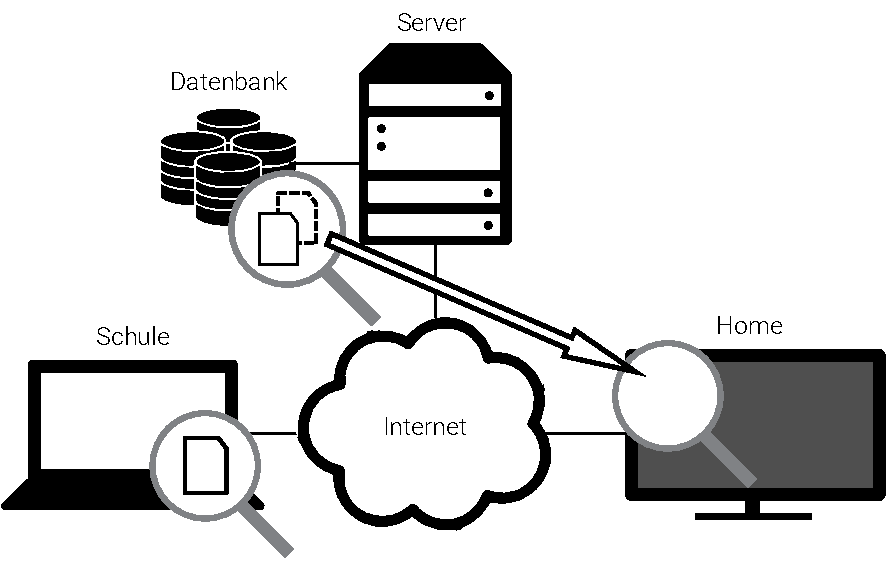
\includegraphics[]{images/dropbox_temp_1}
	\label{dropbox_temp_1}
  \caption{Heimrechner ist nicht erreichbar. Die Datei kann nicht synchronisert werden.}
\end{figure}

\begin{figure}[htb]
	\centering
  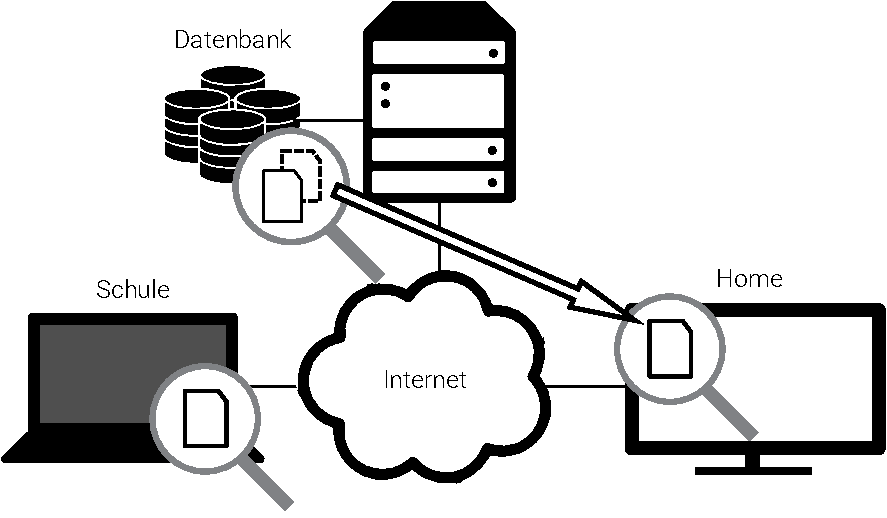
\includegraphics[]{images/dropbox_temp_2}
	\label{dropbox_temp_2}
  \caption{Heimrechner ist wieder erreichbar, sodass die Datei nun vom Server
	bezogen werden kann.}
\end{figure}

Ohne den Server als \gls{filecloud} wäre die alte Version der Datei bearbeitet worden, sodass zwei
neue Versionen der Datei existieren würden. Es wäre also ein \gls{syncconflict} aufgetreten.
%TODO Bild einfügen, auf dem bei sblit ein Client nicht erreichbar ist.
Durch den Verzicht auf den Server muss also eine alternative Lösung gefunden werden,
um Dateien zwischenspeichern und \glspl{syncconflict} vermeiden zu können.

Bei \sblit kommt deshalb eine dezentrale \gls{filecloud} zum Einsatz. Anstelle
der zentralen Speicherung auf einem Server wird zum Zwischenspeichern der Daten eines
Nutzers auf den Speicherplatz auf Geräten anderer Nutzer von \sblit zurückgegriffen.
Die Geräte der Nutzer speichern sich also gegenseitig die Änderungen ihrer Datenbestände
in verlüsselter Form.

Dieses Prinzip funktioniert durch ein \gls{p2pnet}, welches durch faire Abkommen zwischen den \sblit-Nutzern,
sogenannte \glspl{partnership}, realisiert wird. Grundsätzlich sind \glspl{partnership} einfach eine
Vereinbarung mit anderen Nutzern, sich gegenseitig Speicherplatz freizugeben.
Eine \gls{partnership} wird entweder automatisch mit den Geräten unbekannter Nutzer
geschlossen oder durch den Nutzer selbst mit den Geräten bekannter.
Das \kap{Partnerschaften} widmet sich dieser Thematik genauer.

Beim externen Zwischenspeichern auf \glspl{partnerdevice}n sollen diese allerdings
nie vollständigen Zugriff auf fremde Dateien erhalten, welche bei ihnen gespeichert
wurden. Deshalb werden extern zu speichernde Dateien in viele Datenblöcke aufgeteilt.
Diese Blöcke werden verschlüsselt und verstreut auf den \glspl{partnerdevice}n gespeichert.
Die Information zum korrekten Zusammensetzen der Datei besitzen dabei nur der Ersteller selbst und dessen
\glspl{syncpartner}.

Für die Besitzer der \glspl{partnerdevice} ist es somit unmöglich auf die ursprüngliche
Datei zu schließen. Sollte es nämlich einer von ihnen schaffen die Datenblöcke zu
entschlüsseln, würde ihnen noch immer der Rest an Datenblöcken fehlen und die Information
zum korrekten Zusammensetzen dieser.

Von einer ständigen Erreichbarkeit darf auch bei den \glspl{partnerdevice}n nicht
ausgegangen werden. Problematisch wäre es, wenn die Datei nicht von der dezentralen
\gls{filecloud} heruntergeladen werden kann, nur weil eines der \glspl{partnerdevice}
nicht erreichbar ist. Um das zu vermeiden, wird jeder verschlüsselte Datenblock mehrmals
 in der \gls{filecloud} gespeichert, sodass nur ein Bruchteil der
\glspl{partnerdevice} erreichbar sein muss um die komplette Datei anfordern zu können.

Um den Ablauf eines Synchronisationsvorgangs bei \sblit vollständig aufzuzeigen,
folgen nun häufig auftretende Szenarien.

\subsection{Szenarien}
\subsubsection{Allgemein}
Bei \sblit wird der Inhalt eines Ordners synchronisert, der bei der
Erstinstallation der Anwendung angegebenen wurde. Sobald sich Dateien innerhalb des Ordners
ändern, wird die neue Version der Datei kopiert und die Kopie wird den
erreichbaren Synchronisationspartnern über eine direkte verschlüsselte Verbindung
gesendet.

\subsubsection{Synchronisieren bei erreichbaren \glspl{syncpartner}n}
Wenn auf dem Schulrechner eine neue Datei erstellt oder eine bereits synchronisierte verändert und
gespeichert wird, dann wird diese Datei in mehrere Datenblöcke
aufgeteilt, diese Blöcke werden verschlüsselt und direkt über eine verschlüsselte
Verbindung an den Heimrechner gesendet, sofern der jeweilige \gls{syncpartner}
erreichbar ist. Beim \gls{syncpartner} angekommen, werden diese
entschlüsselt und zu der vollständigen neuen Datei zusammengesetzt.

\begin{figure}[htb]
	\centering
  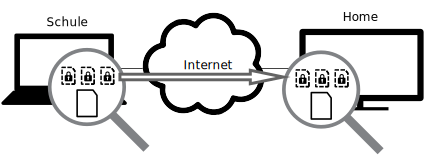
\includegraphics[]{images/sblit_p2p}
	\label{sblit_p2p}
  \caption{Übertragung einer Datei zwischen zwei erreichbaren Hosts.}
\end{figure}

\subsubsection{Synchronisieren bei nicht erreichbaren \glspl{syncpartner}n}
Für \glspl{syncpartner}, die nicht erreichbar sind, wird die Datei in der dezentralen
\gls{filecloud} zwischengespeichert. Die Datei wird kopiert und in Blöcke
aufgeteilt. Diese Blöcke werden verschlüsselt und verteilt auf den
\glspl{partnerdevice}n gespeichert.

Da die Erreichbarkeit der gesamten Datei auf den Partnergeräten zu gewährleisten
ist, wird die Datei mehrmals
in die dezentrale \gls{filecloud} gespeichert, sodass nur ein Bruchteil der
Partnergeräte erreichbar sein muss, um auf die vollständige Datei zugreifen zu
können.

\begin{figure}[htb]
	\centering
  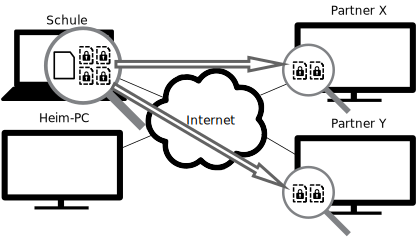
\includegraphics[]{images/sblit_upload}
	\label{sblit_upload}
  \caption{Hochladen einer Datei in die dezentrale \gls{filecloud}.}
\end{figure}

Sobald der \gls{syncpartner}, hier der Heim-PC, wieder hochgefahren ist, fordert er die
verschlüsselten Datenblöcke von den \glspl{partnerdevice}n an. Die Blöcke werden über
direkte verschlüsselte Verbindungen gesendet, entschlüsselt und zu der
vollständigen neuen Datei zusammengesetzt.

\begin{figure}[htb]
	\centering
  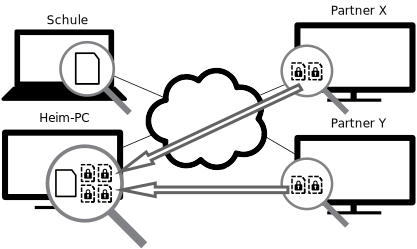
\includegraphics[]{images/sblit_download}
	\label{sblit_download}
  \caption{Herunterladen einer Datei aus der dezentralen \gls{filecloud} beziehungsweise
	von den \glspl{partnerdevice}n.}
\end{figure}
